\chapter{Proposed Method}

{
    Handover in 4G network occurs when a ME move from one cell to another cell.
    And during authentication base station as to confirm ME identity from HSS which
    increase time of handover by twice of propogation delay, twice of transmission delay
    and computation delay (\(2*T_p +2*T_t + T_{c}\)).\\



    In the 4G network, the only part that is wireless is connection between base station
    and ME and range to few kms only. Whereas rest of the connections like BS with MME, 
    MME with HSS is wired and can be thousands of kms appart. Due to which \(T_p\) play a 
    important role in seamless communication.

    \begin{figure}[ht]
        \centering
        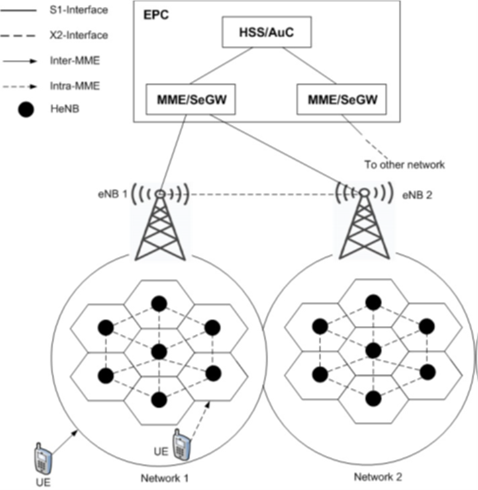
\includegraphics[scale=0.6]{img/celll.png}
        \caption{4G Network Deployment Model}
    \end{figure}

    \section{Assumption Model}{
        The solution for the above problem is given but with few 
        assumption as listed below.
        \begin{itemize}
            \item Only HSS can insert a block in the ledger.
            \item A block is only inserted in the case of intra MME handover.
            \item During intra MME handover \(U_i\) will receive a group key to
             participate in the inter MME handover.
            \item During inter MME handover, user authentication will be done based on
             on the last entry in blockchain as well as the group key.
            \item Once verified user will receive a positive acknowledgement from the
             visited network (BS).
        \end{itemize}

    }

    By keeping this in mind, a solution is proposed in this project. Instead of contacting
    HSS everytime a ME move from one eNB to another eNB. We will only contact HSS in only 2 
    cases:
    \begin{itemize}
        \item When a ME move from one MME to another MME.
        \item If ME dont move from between MME, then after every fixed time interval.
    \end{itemize}
    It doesn't mean we dont have to authenticate ME and eNB during handover. But that process
    of authentication is solely based on the eNB, this method will drastically decrease
    time delay that happens during handover.\\
    \section{Fast and Secure Handover}

    As explained in Chapter 1 for handover will be based on Intra/Inter MME.
    In case of Intra MME handover that is, when a ME move from eNB of one MME to 
    another eNB of different MME, ME with have a
    mutual authentication phase with HSS and then HSS will send a handover key to
    all the eNB in target MME for mutual authentication of ME and eNB. 
    And in case of Inter MME handover, ME stays within the same MME. In this case ME will
    goes through mutual authentication phase with eNB using the handover key that was
    generated previously. After the mutual authentication with eNB in both cases, 
    eNB will create a session key.\\

    This whole process will require credentials which can be extracted from 3 steps:
    \begin{itemize}
        \item Registration of user
        \item Mutual Authentication with HSS
        \item Mutual Authentication with eNB
    \end{itemize}
    In this,step 1 is phase which take place when a SIM is registered to HSS.
    Step 2 and step 3 is part of handover phase. As result it will provide secure
    session key for further data communication.

}


\subsection{Registration of user}{
    When a user want to access 5G technology, user must advance to technology
    which are suitable for protocol of 5G network. For that he must register himself 
    in offile mode. That when he will get Subscription Permanent Indentifier (SUPI).
    But to reduce the threat of information loss we shouldn't use SUPI for communication.
    If in any case SUPI is compromised it will lead to opening a path for the attacker
    to various attacks. So we should use dynamic temporary IDs for further communication.
    In addition to that every new user must register itself with HSS for further authentication.
    So, for solving these two problem a registration request is send to HSS. Then HSS
    will create a Temporary ID (TID) and a random number (r) for the further communication. This will be send
    to user and will be saved in Universal Subscriber Identity Module (USIM).\\
    \begin{figure}[h]
        \centering
        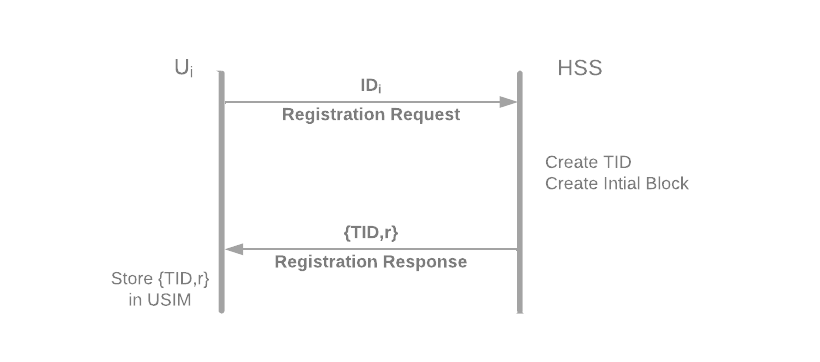
\includegraphics[scale=0.5]{img/res.png}
        \caption{Registration of user in HSS}
    \end{figure}
    \\
    This process can be divied into 3 steps:
    \begin{itemize}
        \item \textbf{Step 1: } {
            User ID (\(ID_i\)) of user \(U_i\) is send in a Registration request to HSS without any encryption as the it send through a trusted channel.
        }
        \item \textbf{Step 2: } {
            Here HSS will have its own secret key (\(k\)) which will not be shared with any other entity.\\

            This following steps will occur here: 
            \begin{itemize}
                \item Collect \(ID_i\)
                \item Select a random number \(r\)
                \item Create \(TID_i\) as \[TID_i = E_k[ID_i||r||T_r]\] , where \(T_r\) is the time stamp of registration of user \(U_i\).
                \item Create Intial Block (\(B_0\)) of the blockchain as \[B_0 = h(ID_i||T_r)\]
                \item With \(ID_i\) store \(T_l \leftarrow \phi\), \(MME_{id} \leftarrow \phi\), \(Blockchain \leftarrow B_0\),
                      where\\ \(T_l\) is time previous handover is taken place\\
                      \(MME_{id}\) is ID of the MME with which \(U_i\) was previous connected with.\\
                      \(Blockchain\) is the blockchain which will store the new block and verify the previously connected nodes.
                \item Send \(TID_i\) and \(r\) to user in Registration Response.
            \end{itemize}
        }
        \item \textbf{Step 3: }{
            Here \(U_i\) will recieve the response and save \(TID_i\) and \(r\)
            in its USIM. That will be for communication later on.
        }
    \end{itemize}

}

\subsection{Mutual Authentication with HSS}{
    Now that registration is complete. Now user will ask for services with 
    service provider. After that whenever user enter a new MME, handover phase will start.
    It happens in steps:
    \begin{itemize}
        \item \textbf{Step 1:}{
            ME will send HSS auth request. To create request these prerequisite is required.
            \begin{itemize}
                \item Create \(K_i\) as, \[K_i = h(ID_i||r)\]
                \item Select another random number \(r_0\)
                \item Create \(R_0\) as, \[R_0 = h(K_i) \oplus r_0 \]
                \item Create \(V_0\) as, \[V_0 = h(ID_i || r_0 || T_u)\] where \(T_u\) is the current time stamp.
                \item Send \(TID_i\), \(R_0\), \(V_0\) and \(T_u\) to HSS via target eNB and target MME.
            \end{itemize}
            Format of the message will be as given below.\\
            
            \begin{table}[h]
                \centering
                \begin{tabular}{|c|c|c|c|c|c|c|}
                    \hline
                    Type & Count & TID & R0 & V0 & Tu & Path\\
                    \hline
                \end{tabular}
                \caption{Format of HSS auth Request}
            \end{table}
            
            Here
            \begin{itemize}
                \item Type will define the type of message it is.
                \item Count will store the jumpt count between the nodes.
                \item TID, R0, V0, Tu are the values which are calculated before.
                \item Path will store the path it will follow to reach HSS
            \end{itemize}
        }
        \item \textbf{Step 2:}{
            Now the HSS auth request has reached the HSS. After that following process
            will take place.
            \begin{itemize}
                \item Verify \(T_u\) with current time stamp. This will help in preventing replay attack.
                \item Decrypt \(TID_i\) with its own secret key (\(k\)), this will give following result \[ID_i||r||T_r = D_k[TID_i]\] Now \(ID_i\), \(r\) and \(T_r\) is extracted from here.
                \item Check if the user is active user or revoked user. It help to identify if the user should get services or not.\\If \[T_u - T_r \le \Delta_{rev},\] then active user
                \item Compute \(K_i\) with values from 2 steps above, as \[K_i = h(ID_i||r)\]
                \item Compute \(r_0\), as \[r_0 = h(K_i) \oplus R_0\]
                \item Verify \(V_0\) by compairing the new \(V_0\) and the \(V_0\) which is received from ME.
                \item Verify previous block of Blockchain.
                \item Create new block of Blockchain as \[B_i = h(B_{i-1}||T_r)\]
                \item Create a temporary factor \(T\) as, \[T = E_k[ID_i||r_i||T_r]\], where \(r_1\) is a new random number
                \item Create new \(TID\), as \[TID_i^{new} = T \oplus h(K_i)\] 
                \item Create handover key (\(hk\)), as \(hk\) is a random hash.
                \item Create \(r^{new}\), as \[r^{new}= h(ID_i||T||r_i||hk||T_h)\] where \(T_h\) is current time stamp
                \item Create \(HK\), as \[HK = h(K_i) \oplus hk \]
                \item Update value in \(ID_i\) as \(T_l \leftarrow T_h\), \(MME_{id} \leftarrow MME_{id}^{prev}\), \(Blockchain \leftarrow B_i\).
            \end{itemize}
        }
        \item \textbf{Step 3:}{
            Now HSS will send 2 messages \\
            \subsubsection*{1st : HSS auth Response}{
                HSS auth Response is send to the ME, with the format as shown below.
                \begin{table}[h]
                    \centering
                    \begin{tabular}{|c|c|c|c|c|c|c|c|c|}
                        \hline
                        Type & Count & ETID & ER & Vi & Tnew & HK & Path & Result\\
                        \hline
                    \end{tabular}
                    \caption{Format of HSS auth Response}
                \end{table}
                \begin{itemize}
                    \item Type will define the type of message it is.
                    \item Count will store the jumpt count between the nodes.
                    \item ETID, ER, Vi, Tnew, HK are the values which are calculated before.
                    \item Path will store the path it will follow to reach HSS
                    \item Result will show if authentication was succeed or not.
                \end{itemize}
            }
            \subsubsection*{2nd : Key Broadcast Request}{
                In this, a key broadcast request is generated in the target MME
                saying that a new ME with \(ID_i\) has enter the network and further
                handover with this ME will be based on the handover key provided here.
                The format of the message is shown below.
                \begin{table}[h]
                    \centering
                    \begin{tabular}{|c|c|c|}
                        \hline
                        Type & ID & hk\\
                        \hline
                    \end{tabular}
                    \caption{Format of Key Broadcast Request}
                \end{table}
            }
        }
        \item \textbf{Step 4:}{
            At the ME side after recieving HSS auth response, following steps is followed.
            \begin{itemize}
                \item Calculate \(K_i\), \(TID_i^{new}\), \(hk\), \(r_i\) from the message values
                \item Using above value verify the \(V_i\).
                \item Store the value in USIM as, \[TID \leftarrow TID_i^{new}, r \leftarrow r_i\]
            \end{itemize}
        }
        \item \textbf{Step 5:}{
            At the MME side who recieved Key Broadcast Request, will send a
            broadcast message to all of its eNB with some modifications as shown below.
            \begin{itemize}
                \item Create \(PID\) as \[PID = h(ID_i||MME_{id}||eNB_{id})\] where \(MME_{id}\) is ID of current MME and \(eNB_{id}\) is the ID of the eNB to which this message is send.
                \item Key Broadcast message to every eNB inside itself. The format of message is shown below.
            \end{itemize}
            \begin{table}[h]
                \centering
                \begin{tabular}{|c|c|c|c|}
                    \hline
                    Type & PID & ID & hk\\
                    \hline
                \end{tabular}
                \caption{Format of Key Broadcast message}
            \end{table}
        }
        \item \textbf{Step 6:}{
            eNB after recieving Key Broadcast message, it will save value of
            \(hk\) and \(PID\) under \(ID_i\).\\
        }
    \end{itemize}
    \begin{figure}[ht]
        \centering
        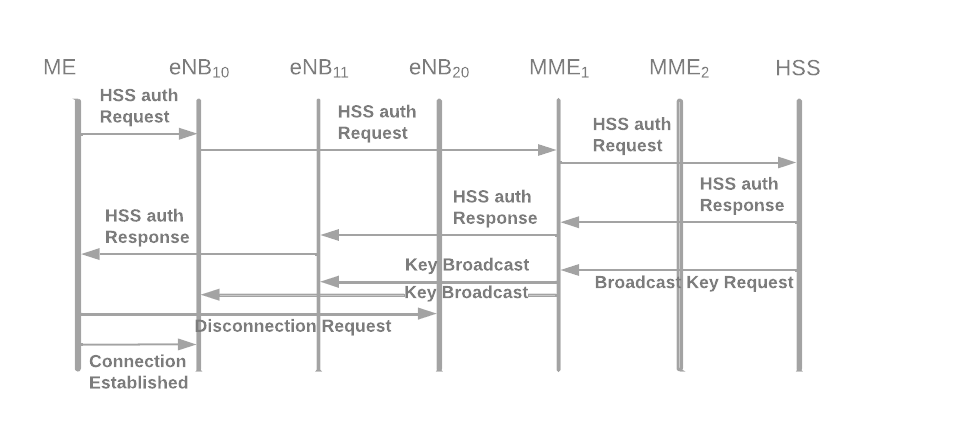
\includegraphics[scale=0.47]{img/hssa.png}
        \caption{Handover from \(eNB_{20}\) to \(eNB_{10}\) )}
    \end{figure}
}

\newpage

\subsection{Mutual Authentication with eNB}{
    The above step will only take place in case of Inter MME handover, but this 
    step will take place in every handover. Here mutual authentication between 
    ME and eNB is designed. For this steps are given below.
    \begin{itemize}
        \item \textbf{Step 1: }{
            Firslty ME will generate a eNB auth request, with following steps:
            \begin{itemize}
                \item Create handover request (\(H_{req}\)) as, \[H_req = E_{hk}[ID_i||T_c]\] where \(T_c\) is current time stamp.
                \item Select a random number \(r_2\)
                \item Create \(V_2\), as \[V_2 = h(ID_i||T_c||r_2)\]
                \item Create \(R_2\), as \[R_2 = r_2 \oplus h(ID_i||T_c)\]
            \end{itemize}
            Now a eNB auth message will be send to eNB with the format as shown below.
            \begin{table}[ht]
                \centering
                \begin{tabular}{|c|c|c|c|}
                    \hline
                    Type & R2 & V2 & Hreq\\
                    \hline
                \end{tabular}
                \caption{Format of eNB auth Request}
            \end{table}
        }
        \\\\
        \item \textbf{Step 2: }{
            At eNB after recieving the eNB auth request, it will authenticate the ME and create a session key for communication with the steps shown below.
            \begin{itemize}
                \item Decrypt \(H_{req}\) with \(hk\) which was given to eNB from its parent MME, giving \[ID_i||T_c = D_{hk}[H_{req}]\]
                \item Verify \(T_c\) with current time stamp
                \item Compute \(r_2\) from \(ID_i\), \(T_c\) and \(R_2\), as \[r_2 = R_2 \oplus h(ID_i||T_v)\]
                \item Verify \(V_2\).
                \item Verify \(PID\)
                \item Select a random number \(r_3\)
                \item Compute \(R_3\), as \[R_3 = r_3 \oplus h(ID_i||T_{hb})\], where \(T_{hb}\) is current time stamp.
                \item Compute \(Hres\), as \[Hres = E_{hk}[ID_i||T_{hb}]\]
                \item Create session key (\(SK\)), as \[SK = h(r2||r3)\]
                \item Send the eNB auth response back to ME with the given format.
            \end{itemize}
            \begin{table}[ht]
                \centering
                \begin{tabular}{|c|c|c|c|}
                    \hline
                    Type & Hres & R3 & Result\\
                    \hline
                \end{tabular}
                \caption{Format of eNB auth Response}
            \end{table}
        }
        \item \textbf{Step 3: }{
            At ME after recieving eNB auth Response, following steps goes on.
            \begin{itemize}
                \item Decrypt \(H_{res}\) with \(hk\), as \[ID_i||T_{hb} = D_{hk}[H_{res}]\]
                \item Verify \(T_{hb}\) with current time stamp.
                \item Compute \(r_3\), as \[r_3 = R_3 \oplus h(ID_i||T_{hb}) \]
                \item Compute session key (\(SK\)), as \[SK = h(r_2||r_3)\]
            \end{itemize}
        }
        \item \textbf{Step 4: }{
        \item Now ME will disconnect with the previous eNB and communicate with new eNB from now using the session key.
        }
        \begin{figure}[ht]
            \centering
            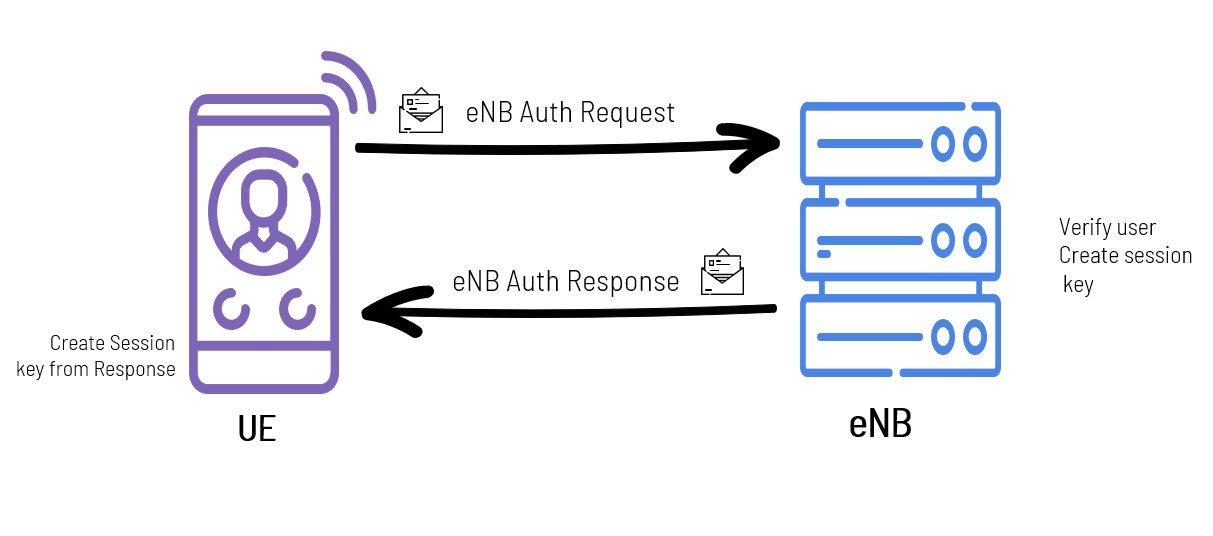
\includegraphics[scale=0.5]{img/enba.jpg}
            \caption{Inter MME Handover}
        \end{figure}
    \end{itemize}
}